
The main objective of the Large Hadron Collider (LHC) was the search for the Brout-Englert-Higgs boson (or scalar boson). It was known from the Linear Electron Positron and Tevatron experiments that the scalar boson mass had to be larger than 114 \si{ \GeV}\cite{Barate:2003sz,Herner:2016woc}, and smaller than around 1 \si{ \TeV} due to unitarity and perturbativity constraints~\cite{Djouadi:2005gi}. On top of this, the search of supersymmetry or dark matter where part of the motivation for building the LHC. 
Since the start of its operation, the LHC is pushing the boundaries of the Standard Model, putting the best limits on physics beyond the Standard Model as well as precision measurements of the parameters of the Standard Model. One such an accomplishment is the discovery the scalar boson in 2012 by the two largest experiments at the LHC~\cite{Chatrchyan:2012xdj,Aad:2012tfa}.

In the first part of this chapter, the LHC and the acceleration process for protons to reach their design energies is discussed. The second part presents the Compact Muon Solenoid. 


\section{The Large Hadron Collider}
The LHC has started its era of cutting edge science on 10 September 2008~\cite{LHC:2008} after approval by the European Organisation of Nuclear Research (CERN) in 1995~\cite{Pettersson:291782}. Installed in the previous Large Electron Positron collider (LEP) tunnels, the LHC consists of a 26.7 $\km$ ring, that is installed between 45 and 170 $\m$ under the French-Swiss border between Cessy (France) and Meyrin (Switzerland). Built to study rare physics phenomena at high energies, the LHC  has the possibility to accelerate two type of particles - protons or ions $Pb^{45+}$ - and provides collisions at four points of interaction. At the interaction points, experiments are installed in order to study the collisions.

 As can be seen in \fig{fig:LHCchain}, the LHC is last element in a chain of creation, injection and acceleration of protons. Protons are obtained by ionising hydrogen and injected in a linear accerator (LINAC 2), where they obtain an energy of 50\si{ \MeV}. They continue to the proton synchrotron booster (PSB or Booster), where the proton packets are accelerated to 1.4\si{ \GeV} and are split up in twelve. The proton synchrotron (PS) increases their energy to 25\si{ \GeV} before handing the protons to the super proton synchrotron (SPS), where the proton reach an energy of 450\si{ \GeV}. Each accelerator ring increases in radius in order to reduce the energy loss of the protons by synchrotron radiation. This energy loss is proportional to the fourth power of the proton energy and inversely proportional to the bending radius. The protons are then injected into opposite directions into the LHC, where they are accelerated to 3.5\si{ \TeV} (in 2010 and 2011), 4\si{ \TeV} (in 2012 and 2013) or 6.5\si{ \TeV} (in 2015 and 2016)~\cite{Wenninger:2254678}. Before the start up of the LHC in 2010, the previous energy record was held by the Tevatron collider at Fermilab, colliding proton with antiprotons at \com = 1.96 \si{ \TeV}.
 
 The beam has a bunch structure obtained by the injection scheme and properties of the dump system. These bunches are obtained in the PS with 25 \si{ \nano \s} spacing. The operation of accelerating and transfering to the LHC is repeated 12 times for each counter-rotating beam.  When completly filled, the LHC nominally contains 2220 bunches in run II, compared to 1380 in run I (design: 2200). At full intensity, it would have nearly 2800 bunches but this is limited due to SPS. 
 
 \begin{figure}[h]
	\centering
	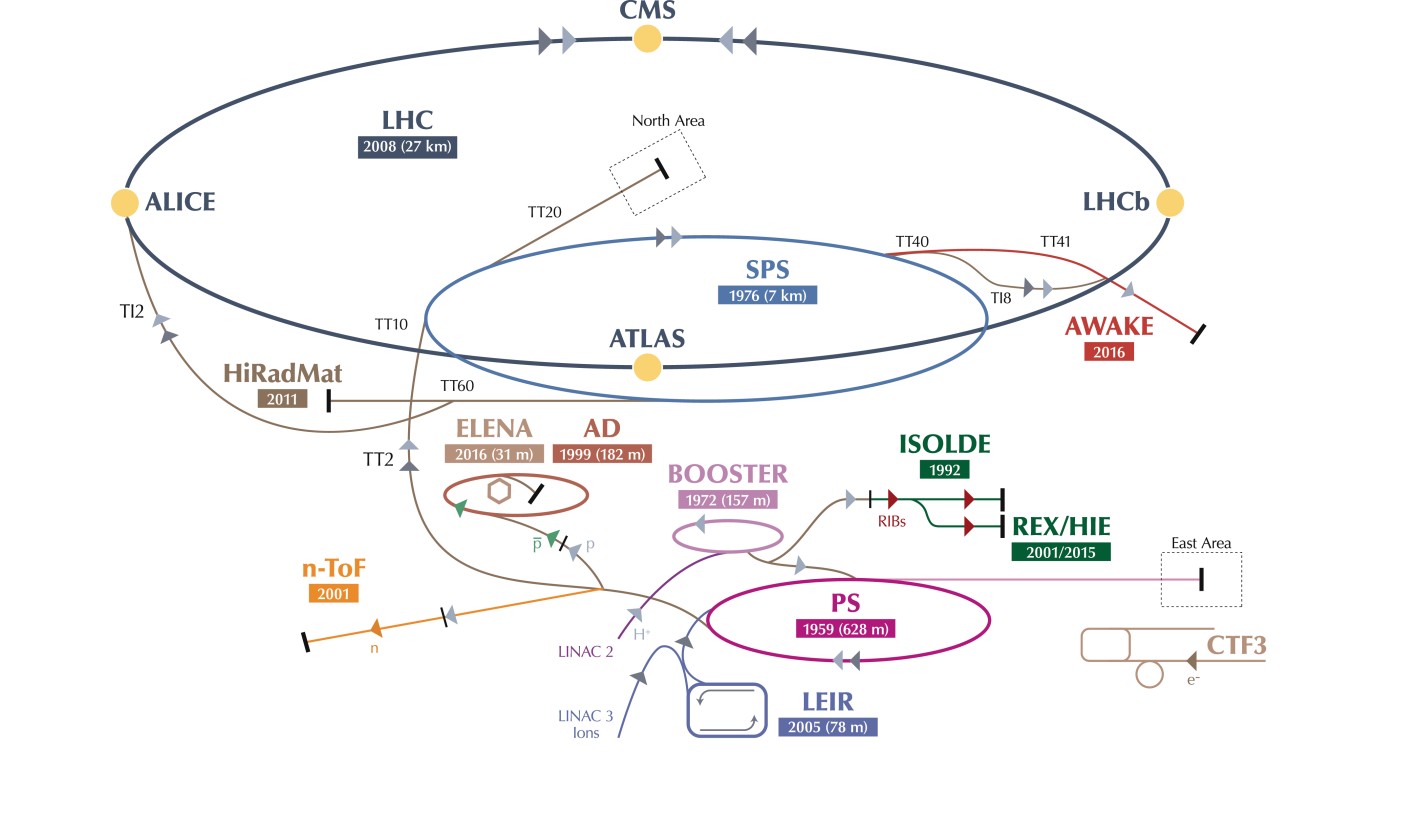
\includegraphics[width=0.75\textwidth]{2_ExperimentalSetup/Figures/CCC-v2016}
	\caption{Schematic representation of the accelerator complex at CERN~\cite{DeMelis:2197559}. The LHC (dark blue) is the last element in chain of accelerators. Protons are successively accelerated by LINAC 2, the Booster, the Proton Synchrotron (PS) and the Super Proton Synchrotron (SPS) before entering the LHC.}
	\label{fig:LHCchain}
\end{figure}

The LHC is home to seven experiments that are placed on an interaction point: 
\begin{itemize}
	\item A Toroidal LHC ApparatuS (ATLAS~\cite{Aad:2008zzm}) and the Compact Muon Solenoid (CMS~\cite{Chatrchyan:2008aa}) experiments are the two general purpose detectors at the LHC. They both have a hermetic, cylindrical structure and were designed to search for new physics phenomena as well as precision measurements of the Standard Model. The existence of two distinct experiments allows cross-confirmation for any discovery. 
	\item A Large Ion Collider Experiment (ALICE~\cite{Aamodt:2008zz}) and the LHC Beauty (LHCb~\cite{Alves:2008zz}) experiments are focusing on specific phenomena. ALICE studies strongly interacting matter at extreme energy densities where quark-gluon plasma forms from heavy ions (Pb-Pb or p-Pb). LHCb searches for differences between matter and anti matter by means of the b quark, while focussing on CP symmetry violation.
	\item The forward LHC (LHCf~\cite{Bongi:2010zz}) and the TOTal cross section, Elastic scattering and diffraction dissociation Measurement (TOTEM~\cite{Anelli:2008zza}) experiments are two smaller experiments that focus on interactions where protons or heavy ions only meet while head on collisions take place. LHCf consists of two parts placed before and after ATLAS and studies particles created at very small angles. TOTEM is placed in the same cavern as CMS and performs precise measurements of the LHC luminosity.
		\item The Monopoles and Exotics Detector At the LHC (MoEDAL~\cite{Acharya:2014nyr}) experiment is situated near LHCb and tries to find magnetic monopoles. 
\end{itemize}


\subsection{LHC design and operation}
 The most important quantity at the LHC is the luminosity\cite{Gillies:1997001}. This is a measurement of the number of collisions that can be produced in a detector per \si{\meter\squared} and per second. The LHC collisions create a number of events per second given by
\begin{equation}\label{eq:NbEv}
\centering
N_{event} = L \sigma_{event}, 
\end{equation}
where $\sigma_{event}$ is the cross section of the event of interest and $L$ the machine luminosity. This luminosity depends only on the beam parameters and is for a Gaussian beam expressed as 
\begin{equation}\label{eq:Lumi}
	L = \frac{1}{4\pi}\textcolor{blue}{N_b n_b f_{rev}}\textcolor{red}{\frac{N_b}{\epsilon_n }}\textcolor{green}{\left(1+\left(\frac{\theta_c \sigma_z}{2\sigma^*} \right)^2\right)^{\frac{-1}{2}}} \frac{\gamma_r}{ \beta^*}.
\end{equation}
The number of particles per bunch is expressed by $N_b$, while $n_b$ is the number of bunches per beam, $f_{rev}$ the revolution frequency, $\gamma_r$ the relativistic gamma factor, $\epsilon_n$ the normalized transverse beam emittance - a quality for the confinement of the beam  , $\beta^*$ the beta function at the collision point - a measurement for the width of the beam, $\theta_c$ the angle between the two beams at the interaction point, $\sigma_z$ the mean lengths of one packet, and $\sigma^*$ the mean height of one packet. In Equation()~\ref{eq:Lumi}), the blue part represents the stream of particles, the red represents the brilliance; and the green part represents the geometric reduction factor due to the crossing angle at the interaction point. 
 Hence, in order to enhance the chances for exploration of rare events and thus enhancing the number of collisions. High beam energies as well as high beam intensities are required.

The peak design luminosity for the LHC in 2016 was $10^{34}$ \si{\per\square\meter \per\second }, which leads to about 1 billion proton interactions per second. In 2016, the LHC was around 10\% above this design luminosity\cite{Harriet:2212301}. The luminosity is not a constant in time. It diminishes due to collisions between the beams, and the interaction of the protons and the particle gas that is trapped in the centre of the vacuum tubes due to the magnetic field. The intern diffusion of the beam degrades the emmitance and therefiore also the luminisity. For this reason, the mean lifetime of a beam inside the LHC is around 15 \si{ \hour}. The integrated luminosity - the luminosity provided for a certain time range - recorded by CMS and ATLAS over the year 2016 is given in \fig{fig:IntLumi}. In Run II, the peak luminosity is 13-17 10$^33$ \si{ \per \square \centi \meter \per \second} compared to 7.7 10$^33$ \si{ \per \square \centi \meter \per \second} in Run I.
% https://science.energy.gov/~/media/hep/hepap/pdf/201512/CMSRestart_Rakness_HEPAP_20151210.pdf
 \begin{figure}[ht]
 	\centering
	\begin{minipage}[b]{0.4\textwidth}
	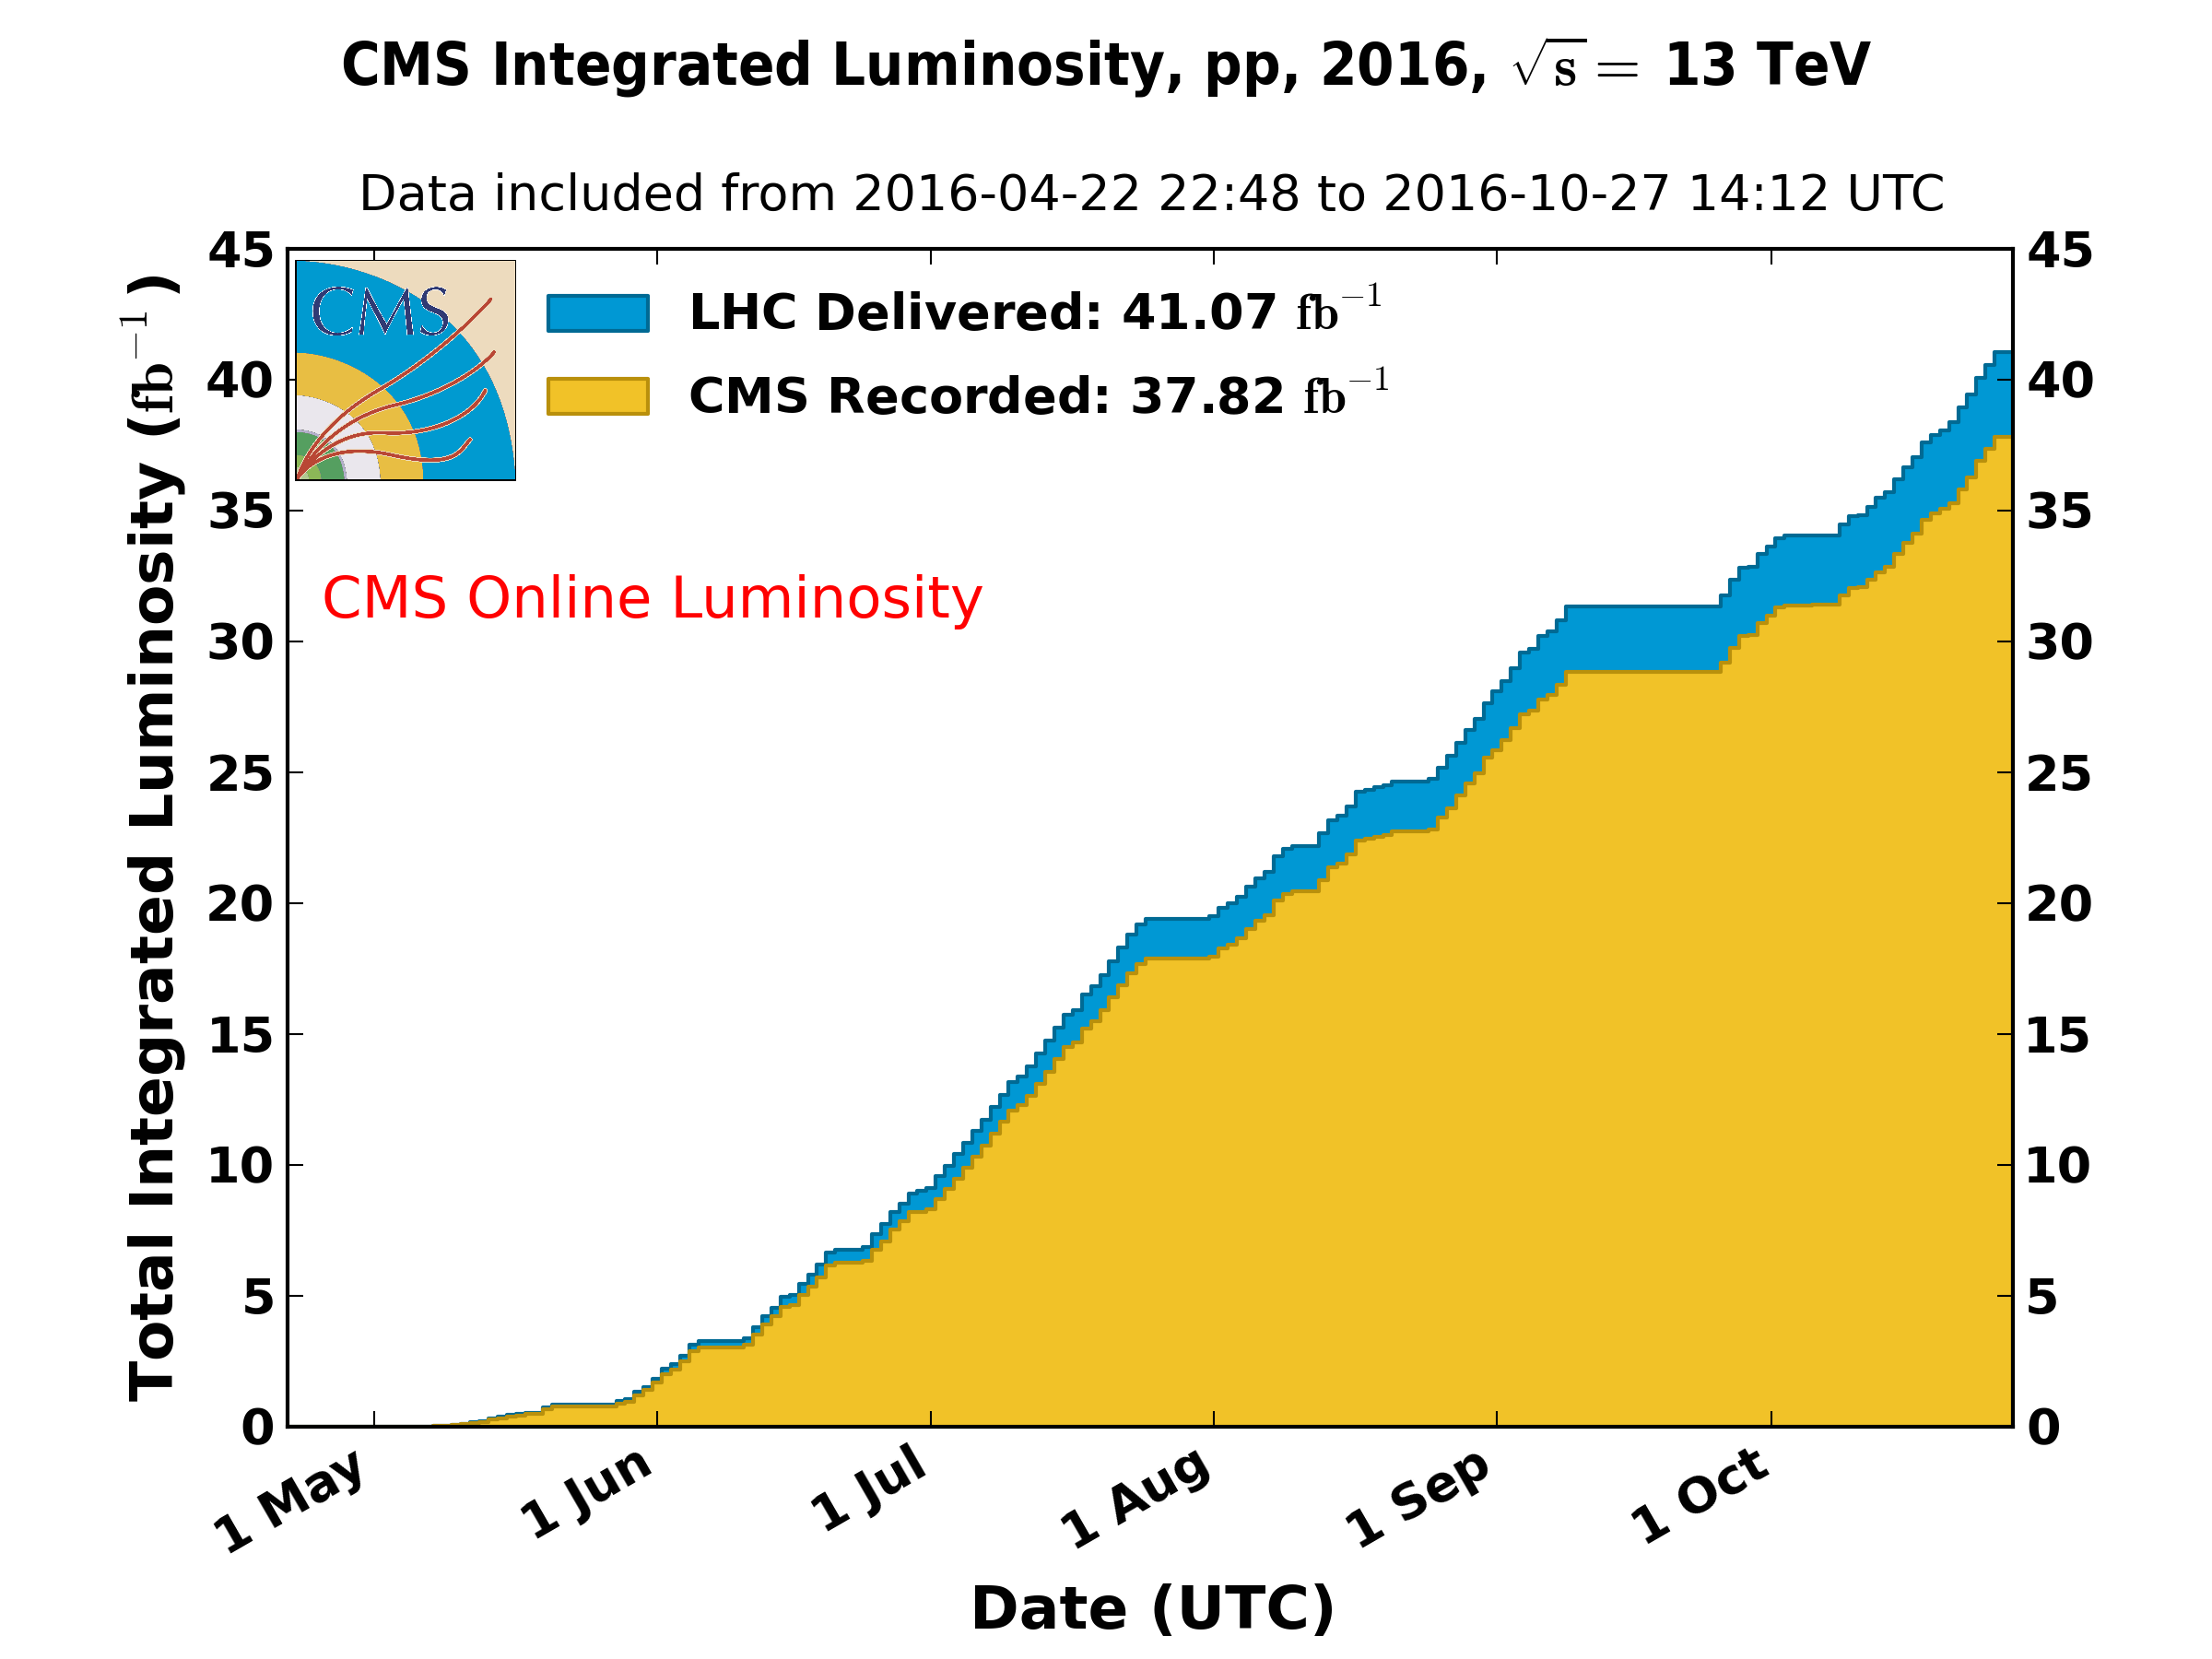
\includegraphics[width=\textwidth]{2_ExperimentalSetup/Figures/int_lumi_per_day_cumulative_pp_2016OnlineLumi}
	\caption{Cumulative luminosity measured online versus day delivered to (blue), and recorded by CMS (orange) during stable beams and for proton collisions at 13 TeV centre-of-mass energy in 2016. The delivered luminosity accounts for the luminosity delivered from the start of stable beams until the LHC requests CMS to turn off the sensitive detectors to allow a beam dump or beam studies. FIXME}
    \end{minipage}
\hfill
\begin{minipage}[b]{0.4\textwidth}
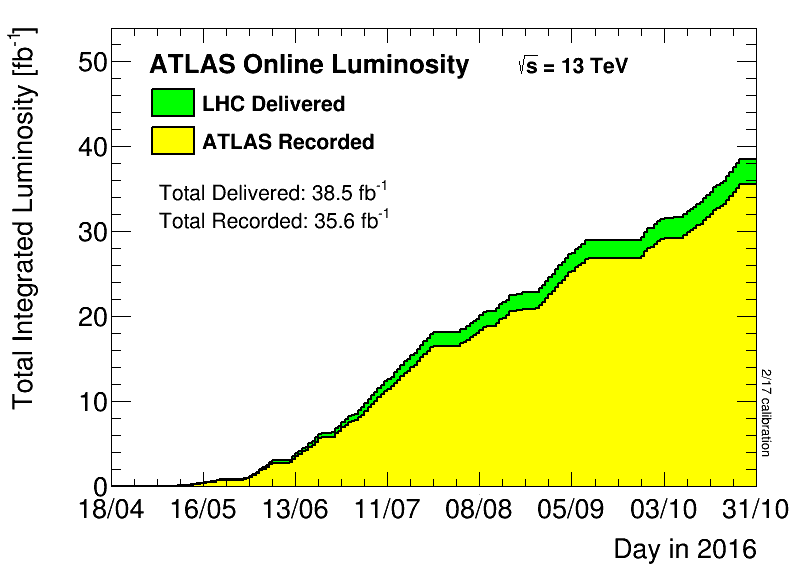
\includegraphics[width=\textwidth]{2_ExperimentalSetup/Figures/sumLumiByDay}
	\caption{Total Integrated Luminosity in 2016 
		Cumulative luminosity versus time delivered to (green) and recorded by ATLAS (yellow) during stable beams for proton collisions  in 2016. The delivered luminosity accounts for luminosity delivered from the start of stable beams until the LHC requests ATLAS to put the detector in a safe standby mode to allow for a beam dump or beam studies. Shown is the luminosity as determined from counting rates measured by the luminosity detectors. FIXME}
	\end{minipage}
	\label{fig:IntLumi}
%	(from https://twiki.cern.ch/twiki/bin/view/CMSPublic/LumiPublicResults#Online_Luminosity_AN2 )
\end{figure}

 
Inside the LHC ring~\cite{Bruning:782076}, the protons are accelerated by the means of radiofrequenciy cavities, while 1232  magnets of approximately 15\si{ \m} long, weighing 35\si{ \tonne} esure the deflection of the beams. The cross section view of such a dipole is given in \fig{fig:dipole}. The two proton beams circulate in opposite direction in separate pipes inside of the magnet. Through the use of a strong electric current in the coils around the beam pipe, magnetic fields are generated and cause the protons to bend in the required orbits. In order to get the coil to become superconducting and able to produce - with the aid of an iron return yoke - a strong magnetic field of 8.3\si{ \tesla}, the magnet structure is surrounded by a vessel. This vessel is filled with liquid Helium making it possible to cool down the magnet to 1.9\si{ \kelvin}. In order to get more focussed and stabilised proton beam, other higher-order multipole and corrector magnets are placed along the LHC tunnel.

 \begin{figure}[ht]
	\centering
	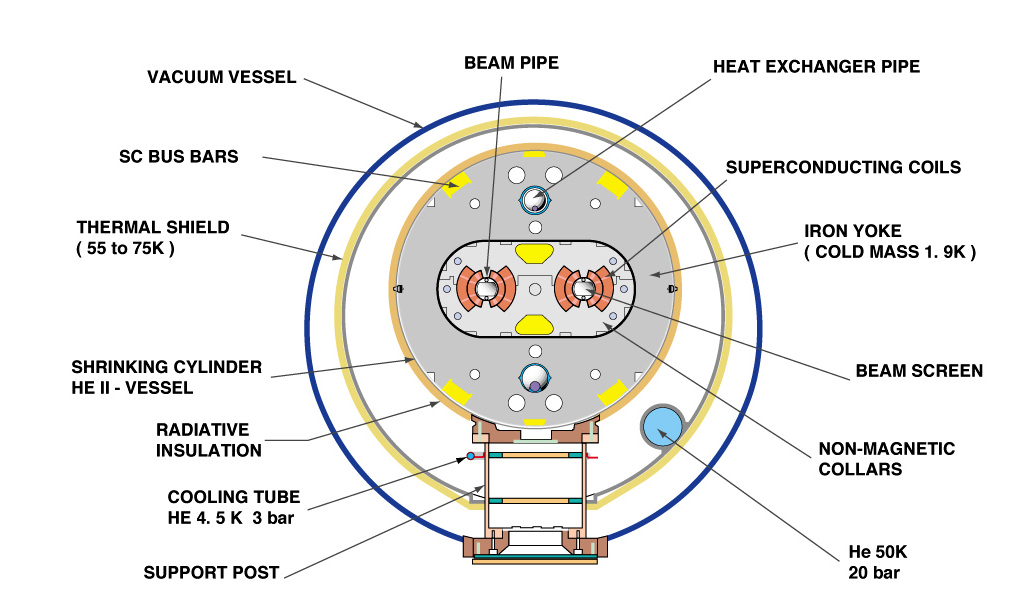
\includegraphics[width=0.45\textwidth]{2_ExperimentalSetup/Figures/lhc-pho-1998-341}
%	\includegraphics[width=0.45\textwidth]{2_ExperimentalSetup/Figures/1107167_03}
	\caption{Schematic representation of the LHC dipole~\cite{Jean-Luc:841539} . Two beam pipes where the proton beams circulate around the LHC ring are shown. The superconducting coils generate a magnetic field of 8.3 \tesla that steer the protons in the circular path. }
	\label{fig:dipole}
\end{figure}




%CMS collaboration http://cds.cern.ch/record/2195940?ln=en map
